\section{Direction of Arrival with FDOA Measurements}
\label{s:FDOA}

Consider a stationary transmitter located at $\mbf{x}$. Suppose we have $N$ receivers located at $\mbf{x}_1, ...,\mbf{x}_N$ with velocities $\mbf{v}_1, ...,\mbf{v}_N$. The frequency shift of the signal between the emitter and the $i^{th}$ receiver is
\begin{align}
  \label{eq:fshift}
  d_i =  \frac{f_0}{c}\left(\mbf{v}_i^T\cdot\frac{\mbf{x}_i-\mbf{x}}{\|\mbf{x}_i-\mbf{x}\|}\right),
\end{align}
where $f_0$ is the emitted frequency and $c$ is the speed of wave propagation in the media. In our scenario, we know the receiver positions and velocities, and we would like to solve for the transmitter position. We cannot measure the frequency shift directly, but we can measure the difference in frequency shifts,
$f_{i,j} = d_j-d_i$. Scaling by $\|\mbf{x}_i-\mbf{x}\|^{-1}$ means that each of these equations is nonlinear. Even so, by taking pairwise differences of the equations in \eqref{eq:fshift}, one can numerically solve the system by expressing it in terms of polynomials and using techniques like homotopy continuation \cite{Cameron}. While such an approach is able to find all solutions, it is computationally more expensive than a linear solve.

The nonlinearity of \eqref{eq:fshift} makes it difficult to accurately solve for $\mbf{x}$, so we simplify the model by deriving a far-field approximation for Equation \ref{eq:fshift}. Additionally, for simplicity we ignore the constant factor of $f_0/c$ in~\eqref{eq:fshift}. Thus $d_i$ is now \textit{proportional} to the frequency shift.

\subsection{Far-field Approximation for FDOA}
Assume without loss of generality that the receivers are centered around the origin. We consider the far-field case, where the distance between receivers is much smaller than the distance to the emitter, i.e. $\|\mathbf{x}-\mathbf{x}_i\|>>\|\mathbf{x}_i\|, \; \forall \; i$. The far-field approximation (as in~\cite{Cheney2009}) for $1/\|\mathbf{x-x_i}\|$ is:
\begin{align*}
  \frac{1}{\|\mathbf{x-x_i}\|} = \frac{1}{\|\mathbf{x}\|}\left(1+\mathcal{O}\left(\frac{\|\mathbf{x}_i\|}{\|\mathbf{x}\|}\right)\right).
\end{align*}
Truncating after the first term above allows for simplification of the factor (in eq. \ref{eq:fshift}):
\begin{align*}
  \frac{\mbf{x}_i-\mbf{x}}{\|\mbf{x}_i-\mbf{x}\|} \approx \frac{\mbf{x}_i}{\|\mbf{x}\|}-\frac{\mbf{x}}{\|\mbf{x}\|}.
\end{align*}
Additionally, the far-field assumption implies that the first term will have small magnitude. Thus, $\dfrac{\mathbf{x_i-x}}{\|\mathbf{x_i-x}\|}$ is simplified to $\dfrac{-\mathbf{x}}{\|\mathbf{x}\|}$.
Equation \ref{eq:fshift} becomes:
\begin{align}
  d_i =  -\mbf{v}_i^T\cdot\hat{\mbf{x}},
\end{align}
where $\hat{\mbf{x}} = \frac{\mbf{x}}{\|\mbf{x}\|}$, is the unit vector in the direction of $\mbf{x}$. The entire system of frequency shifts can be written:
\begin{align}
  \label{eq:fshiftFF}
\mbf{d} = -\mbf{V}\hat{\mbf{x}},
\end{align}
where \begin{align*}
\mathbf{d}=\begin{pmatrix}
d_1 \\ \vdots \\ d_N
\end{pmatrix}
\qquad
\mathbf{V}=\begin{pmatrix}
\mathbf{v}_1^T \\ \vdots\\ \mathbf{v}_N^T
\end{pmatrix}.
\end{align*}

In practice, the frequency shifts are not observable. Instead the frequency difference of arrival (FDOA) is measured between receivers. The FDOA is equivalent to the difference in frequency shifts,
\begin{align}
  \label{eq:fdoa}
  f_{i,j} = d_j-d_i.
\end{align}
A system equivalent to Equation \eqref{eq:fshiftFF} can be constructed for the FDOA, with the use of a differencing matrix $\mbf{P}$. The matrix $\mbf{P}$ has entries of 0 and $\pm 1$ corresponding to the differencing in Equation \eqref{eq:fdoa}. Thus, with the far-field simplification above, the vector of FDOA measurements, $\mbf{f}$, is equivalent to,
\begin{align}
  \label{eq:fdoaFF}
\mbf{f} = -\mbf{PV}\hat{\mbf{x}}.
\end{align}
The matrix $\mbf{-PV}$ will be referred to as $\tilde{\mbf{V}}$ for simplicity.

This far-field simplification reduces the FDOA equations to a linear system. This suggests that feasible FDOA measurements in the far-field case lie on the image of the unit circle transformed by the matrix $\tilde{\mbf{V}}$. This image is an ellipse with rotation and scaling determined by the singular value decomposition of $\tilde{\mbf{V}}$. Indeed, this can be confirmed by computing the singular value decomposition of generated far-field FDOA measurements and confirming they lie on the same subspace as $\tilde{\mbf{V}}$. This relationship can be demonstrated visually with a plot of generated FDOA measurements (Fig. \ref{f:ellipse}).

\begin{figure}[h!]
  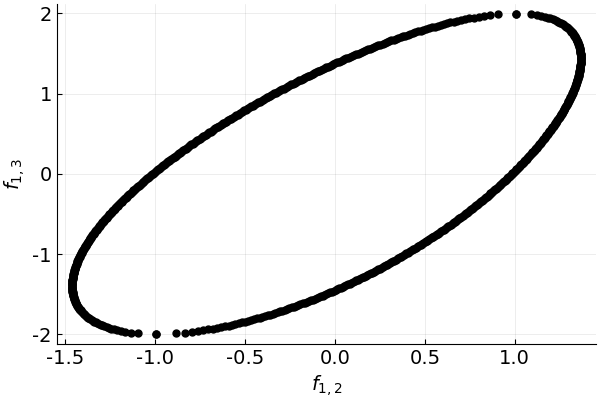
\includegraphics[scale=0.7]{FDOAellipse.png}
  \caption{Plot of far-field $f_{1,2}$ vs. $f_{1,3}$ for a system of three receivers centered around the origin. Note the image is an ellipse with scaling in the direction of the left-singular vectors of $\tilde{\mbf{V}}$.}
  \label{f:ellipse}
\end{figure}


\subsection{Calculating direction of arrival (DOA)}
The far-field approximated form of the FDOA equations is linear with variable $\hat{\mbf{x}}$, representing the direction of arrival (DOA) of the signal. Thus, the DOA can be found by solving \eqref{eq:fdoaFF} for $\hat{\mbf{x}}$. If there are more FDOA measurements than direction components, we can find the least squares solution to the problem, which is also the pseudo-inverse solution:
\begin{align}
  \label{eq:doa}
\hat{\mbf{x}} = (\tilde{\mbf{V}}^T\tilde{\mbf{V}})^{-1}\tilde{\mbf{V}}^T\mathbf{f}.
\end{align}

One method for denoising in TDOA-based geolocation is the projection of noisy measurements onto the range of the differencing matrix $\mathbf{P}$~\cite{Schmidt1996,Compagnoni2017}. This ensures that the TDOA measurements are physically realizable and consistent between receivers. One benefit of the method for DOA calculation proposed above is that denoising is automatically performed since projection onto the range of $\mathbf{-PV}$ is equivalent to projection onto the range of $\mathbf{P}$.
